\documentclass{standalone}
\usepackage{tikz}
\usetikzlibrary{patterns}
\usetikzlibrary{positioning}
\usetikzlibrary{patterns, positioning}
\usetikzlibrary{shapes.misc}
\usepackage[outline]{contour}
\contourlength{1.5pt} 
\usetikzlibrary{calc}
        \usepackage{relsize}
        \tikzset{fontscale/.style = {font=\relsize{#1}}}

\begin{document}
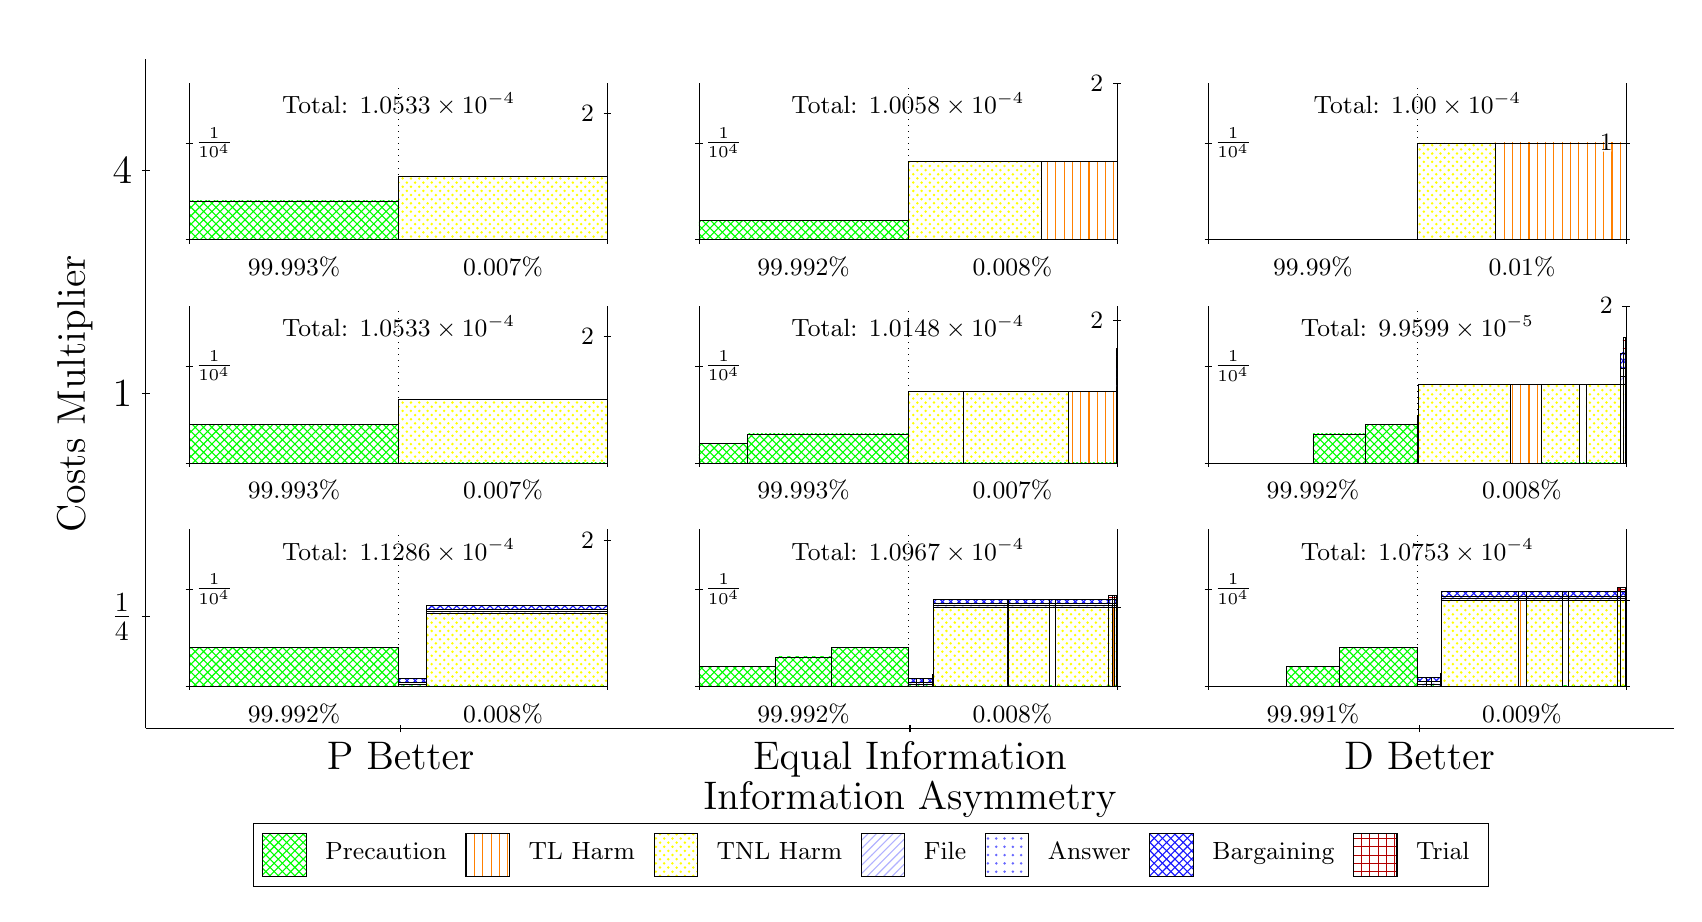
\begin{tikzpicture}
\clip(-0.5,-1.1) rectangle +(20.91,11);
\draw[black] (1,1) -- (1,9.5);
\node[rotate=90, fontscale=2, anchor=center] at (0.1, 5.25) {Costs Multiplier};
\draw[black] (0.95,2.4167) -- (1.05,2.4167);
\node[fontscale=2, anchor=east] at (0.95, 2.4167) {$\frac{1}{4}$};
\draw[black] (0.95,5.25) -- (1.05,5.25);
\node[fontscale=2, anchor=east] at (0.95, 5.25) {1};
\draw[black] (0.95,8.0833) -- (1.05,8.0833);
\node[fontscale=2, anchor=east] at (0.95, 8.0833) {4};

\draw[black] (1,1) -- (20.41,1);
\node[fontscale=2, anchor=center] at (10.705, 0.1) {Information Asymmetry};
\draw[black] (4.235,0.95) -- (4.235,1.05);
\node[fontscale=2, anchor=north] at (4.235, 0.95) {P Better};
\draw[black] (10.705,0.95) -- (10.705,1.05);
\node[fontscale=2, anchor=north] at (10.705, 0.95) {Equal Information};
\draw[black] (17.175,0.95) -- (17.175,1.05);
\node[fontscale=2, anchor=north] at (17.175, 0.95) {D Better};


\draw[pattern=crosshatch, pattern color=green,draw=black,very thin] (1.5556,1.54) rectangle (4.21,2.032);
\draw[pattern=crosshatch, pattern color=green,draw=black,very thin] (4.21,1.54) rectangle (4.5624,1.54);
\draw[pattern=north east lines, pattern color=blue!30,draw=black,very thin] (4.21,1.54) rectangle (4.5624,1.5632);
\draw[pattern=dots,  pattern color=blue!60,draw=black,very thin] (4.21,1.5632) rectangle (4.5624,1.5864);
\draw[pattern=crosshatch,      pattern color=blue!90,draw=black,very thin] (4.21,1.5864) rectangle (4.5624,1.6327);
\draw[pattern=crosshatch, pattern color=green,draw=black,very thin] (4.5624,1.54) rectangle (6.8644,1.54);
\draw[pattern=crosshatch dots, pattern color=yellow,draw=black,very thin] (4.5624,1.54) rectangle (6.8644,2.4667);
\draw[pattern=north east lines, pattern color=blue!30,draw=black,very thin] (4.5624,2.4667) rectangle (6.8644,2.4898);
\draw[pattern=dots,  pattern color=blue!60,draw=black,very thin] (4.5624,2.4898) rectangle (6.8644,2.513);
\draw[pattern=crosshatch,      pattern color=blue!90,draw=black,very thin] (4.5624,2.513) rectangle (6.8644,2.5593);
\node[font=\small,text=black,anchor=north] at (4.21, 3.5333) {Total: $1.1286\times 10^{-4}$};
\draw[black,very thin] (1.5556,1.54) -- (1.5556,3.5333);
\draw[black,very thin] (1.5056,1.54) -- (1.6056,1.54);
\node[font=\small,text=black, anchor=west] at (1.5056, 1.54) {};
\draw[black,very thin] (1.5056,2.7701) -- (1.6056,2.7701);
\node[font=\small,text=black, anchor=west] at (1.5056, 2.7701) {$\frac{1}{10^{4}}$};

\draw[black,dotted,very thin] (4.21,1.5998) -- (4.21,3.4735);
\draw[black,very thin] (6.8644,1.54) -- (6.8644,3.5333);
\draw[black,very thin] (6.8144,3.3933) -- (6.9144,3.3933);
\node[font=\small,text=black, anchor=east] at (6.8144, 3.3933) {\contour{white}{2}};

\draw[black,very thin] (1.5556,1.54) -- (6.8644,1.54);
\draw[black,very thin] (1.5556,1.49) -- (1.5556,1.59);
\node[font=\small,text=black, anchor=north] at (1.5556, 1.49) {};
\draw[black,very thin] (6.8644,1.49) -- (6.8644,1.59);
\node[font=\small,text=black, anchor=north] at (6.8644, 1.49) {};

\node[font=\small,text=black,anchor=south] at (2.8828, 0.94) {99.992\%};
\node[font=\small,text=black,anchor=south] at (5.5372, 0.94) {0.008\%};

\draw[pattern=crosshatch, pattern color=green,draw=black,very thin] (8.0256,1.54) rectangle (8.9948,1.786);
\draw[pattern=crosshatch, pattern color=green,draw=black,very thin] (8.9948,1.54) rectangle (9.7108,1.909);
\draw[pattern=crosshatch, pattern color=green,draw=black,very thin] (9.7108,1.54) rectangle (10.68,2.032);
\draw[pattern=crosshatch, pattern color=green,draw=black,very thin] (10.68,1.54) rectangle (10.79,1.54);
\draw[pattern=north east lines, pattern color=blue!30,draw=black,very thin] (10.68,1.54) rectangle (10.79,1.565);
\draw[pattern=dots,  pattern color=blue!60,draw=black,very thin] (10.68,1.565) rectangle (10.79,1.5901);
\draw[pattern=crosshatch,      pattern color=blue!90,draw=black,very thin] (10.68,1.5901) rectangle (10.79,1.6401);
\draw[pattern=crosshatch, pattern color=green,draw=black,very thin] (10.79,1.54) rectangle (10.873,1.54);
\draw[pattern=north east lines, pattern color=blue!30,draw=black,very thin] (10.79,1.54) rectangle (10.873,1.565);
\draw[pattern=dots,  pattern color=blue!60,draw=black,very thin] (10.79,1.565) rectangle (10.873,1.5901);
\draw[pattern=crosshatch,      pattern color=blue!90,draw=black,very thin] (10.79,1.5901) rectangle (10.873,1.6401);
\draw[pattern=crosshatch, pattern color=green,draw=black,very thin] (10.873,1.54) rectangle (10.992,1.54);
\draw[pattern=north east lines, pattern color=blue!30,draw=black,very thin] (10.873,1.54) rectangle (10.992,1.5651);
\draw[pattern=dots,  pattern color=blue!60,draw=black,very thin] (10.873,1.5651) rectangle (10.992,1.5901);
\draw[pattern=crosshatch,      pattern color=blue!90,draw=black,very thin] (10.873,1.5901) rectangle (10.992,1.6401);
\draw[pattern=crosshatch, pattern color=green,draw=black,very thin] (10.992,1.54) rectangle (11.001,1.54);
\draw[pattern=north east lines, pattern color=blue!30,draw=black,very thin] (10.992,1.54) rectangle (11.001,1.565);
\draw[pattern=dots,  pattern color=blue!60,draw=black,very thin] (10.992,1.565) rectangle (11.001,1.5901);
\draw[pattern=crosshatch,      pattern color=blue!90,draw=black,very thin] (10.992,1.5901) rectangle (11.001,1.6401);
\draw[pattern=grid,            pattern color=red!70!black,draw=black,very thin] (10.992,1.6401) rectangle (11.001,1.6901);
\draw[pattern=crosshatch, pattern color=green,draw=black,very thin] (11.001,1.54) rectangle (11.006,1.54);
\draw[pattern=north east lines, pattern color=blue!30,draw=black,very thin] (11.001,1.54) rectangle (11.006,1.565);
\draw[pattern=dots,  pattern color=blue!60,draw=black,very thin] (11.001,1.565) rectangle (11.006,1.5901);
\draw[pattern=crosshatch,      pattern color=blue!90,draw=black,very thin] (11.001,1.5901) rectangle (11.006,1.6401);
\draw[pattern=grid,            pattern color=red!70!black,draw=black,very thin] (11.001,1.6401) rectangle (11.006,1.6901);
\draw[pattern=crosshatch, pattern color=green,draw=black,very thin] (11.006,1.54) rectangle (11.939,1.54);
\draw[pattern=crosshatch dots, pattern color=yellow,draw=black,very thin] (11.006,1.54) rectangle (11.939,2.5407);
\draw[pattern=north east lines, pattern color=blue!30,draw=black,very thin] (11.006,2.5407) rectangle (11.939,2.5657);
\draw[pattern=dots,  pattern color=blue!60,draw=black,very thin] (11.006,2.5657) rectangle (11.939,2.5907);
\draw[pattern=crosshatch,      pattern color=blue!90,draw=black,very thin] (11.006,2.5907) rectangle (11.939,2.6408);
\draw[pattern=crosshatch, pattern color=green,draw=black,very thin] (11.939,1.54) rectangle (11.949,1.54);
\draw[pattern=vertical lines, pattern color=orange,draw=black,very thin] (11.939,1.54) rectangle (11.949,2.5407);
\draw[pattern=north east lines, pattern color=blue!30,draw=black,very thin] (11.939,2.5407) rectangle (11.949,2.5657);
\draw[pattern=dots,  pattern color=blue!60,draw=black,very thin] (11.939,2.5657) rectangle (11.949,2.5907);
\draw[pattern=crosshatch,      pattern color=blue!90,draw=black,very thin] (11.939,2.5907) rectangle (11.949,2.6408);
\draw[pattern=crosshatch, pattern color=green,draw=black,very thin] (11.949,1.54) rectangle (12.476,1.54);
\draw[pattern=crosshatch dots, pattern color=yellow,draw=black,very thin] (11.949,1.54) rectangle (12.476,2.5407);
\draw[pattern=north east lines, pattern color=blue!30,draw=black,very thin] (11.949,2.5407) rectangle (12.476,2.5657);
\draw[pattern=dots,  pattern color=blue!60,draw=black,very thin] (11.949,2.5657) rectangle (12.476,2.5907);
\draw[pattern=crosshatch,      pattern color=blue!90,draw=black,very thin] (11.949,2.5907) rectangle (12.476,2.6408);
\draw[pattern=crosshatch, pattern color=green,draw=black,very thin] (12.476,1.54) rectangle (12.547,1.54);
\draw[pattern=vertical lines, pattern color=orange,draw=black,very thin] (12.476,1.54) rectangle (12.547,2.5407);
\draw[pattern=north east lines, pattern color=blue!30,draw=black,very thin] (12.476,2.5407) rectangle (12.547,2.5657);
\draw[pattern=dots,  pattern color=blue!60,draw=black,very thin] (12.476,2.5657) rectangle (12.547,2.5907);
\draw[pattern=crosshatch,      pattern color=blue!90,draw=black,very thin] (12.476,2.5907) rectangle (12.547,2.6408);
\draw[pattern=crosshatch, pattern color=green,draw=black,very thin] (12.547,1.54) rectangle (13.226,1.54);
\draw[pattern=crosshatch dots, pattern color=yellow,draw=black,very thin] (12.547,1.54) rectangle (13.226,2.5407);
\draw[pattern=north east lines, pattern color=blue!30,draw=black,very thin] (12.547,2.5407) rectangle (13.226,2.5657);
\draw[pattern=dots,  pattern color=blue!60,draw=black,very thin] (12.547,2.5657) rectangle (13.226,2.5908);
\draw[pattern=crosshatch,      pattern color=blue!90,draw=black,very thin] (12.547,2.5908) rectangle (13.226,2.6408);
\draw[pattern=crosshatch, pattern color=green,draw=black,very thin] (13.226,1.54) rectangle (13.28,1.54);
\draw[pattern=crosshatch dots, pattern color=yellow,draw=black,very thin] (13.226,1.54) rectangle (13.28,2.5407);
\draw[pattern=north east lines, pattern color=blue!30,draw=black,very thin] (13.226,2.5407) rectangle (13.28,2.5657);
\draw[pattern=dots,  pattern color=blue!60,draw=black,very thin] (13.226,2.5657) rectangle (13.28,2.5907);
\draw[pattern=crosshatch,      pattern color=blue!90,draw=black,very thin] (13.226,2.5907) rectangle (13.28,2.6408);
\draw[pattern=grid,            pattern color=red!70!black,draw=black,very thin] (13.226,2.6408) rectangle (13.28,2.6908);
\draw[pattern=crosshatch, pattern color=green,draw=black,very thin] (13.28,1.54) rectangle (13.297,1.54);
\draw[pattern=vertical lines, pattern color=orange,draw=black,very thin] (13.28,1.54) rectangle (13.297,2.5407);
\draw[pattern=north east lines, pattern color=blue!30,draw=black,very thin] (13.28,2.5407) rectangle (13.297,2.5657);
\draw[pattern=dots,  pattern color=blue!60,draw=black,very thin] (13.28,2.5657) rectangle (13.297,2.5907);
\draw[pattern=crosshatch,      pattern color=blue!90,draw=black,very thin] (13.28,2.5907) rectangle (13.297,2.6408);
\draw[pattern=grid,            pattern color=red!70!black,draw=black,very thin] (13.28,2.6408) rectangle (13.297,2.6908);
\draw[pattern=crosshatch, pattern color=green,draw=black,very thin] (13.297,1.54) rectangle (13.321,1.54);
\draw[pattern=crosshatch dots, pattern color=yellow,draw=black,very thin] (13.297,1.54) rectangle (13.321,2.5407);
\draw[pattern=north east lines, pattern color=blue!30,draw=black,very thin] (13.297,2.5407) rectangle (13.321,2.5657);
\draw[pattern=dots,  pattern color=blue!60,draw=black,very thin] (13.297,2.5657) rectangle (13.321,2.5907);
\draw[pattern=crosshatch,      pattern color=blue!90,draw=black,very thin] (13.297,2.5907) rectangle (13.321,2.6408);
\draw[pattern=grid,            pattern color=red!70!black,draw=black,very thin] (13.297,2.6408) rectangle (13.321,2.6908);
\draw[pattern=crosshatch, pattern color=green,draw=black,very thin] (13.321,1.54) rectangle (13.334,1.54);
\draw[pattern=vertical lines, pattern color=orange,draw=black,very thin] (13.321,1.54) rectangle (13.334,2.5407);
\draw[pattern=north east lines, pattern color=blue!30,draw=black,very thin] (13.321,2.5407) rectangle (13.334,2.5657);
\draw[pattern=dots,  pattern color=blue!60,draw=black,very thin] (13.321,2.5657) rectangle (13.334,2.5907);
\draw[pattern=crosshatch,      pattern color=blue!90,draw=black,very thin] (13.321,2.5907) rectangle (13.334,2.6408);
\draw[pattern=grid,            pattern color=red!70!black,draw=black,very thin] (13.321,2.6408) rectangle (13.334,2.6908);
\node[font=\small,text=black,anchor=north] at (10.68, 3.5333) {Total: $1.0967\times 10^{-4}$};
\draw[black,very thin] (8.0256,1.54) -- (8.0256,3.5333);
\draw[black,very thin] (7.9756,1.54) -- (8.0756,1.54);
\node[font=\small,text=black, anchor=west] at (7.9756, 1.54) {};
\draw[black,very thin] (7.9756,2.7701) -- (8.0756,2.7701);
\node[font=\small,text=black, anchor=west] at (7.9756, 2.7701) {$\frac{1}{10^{4}}$};

\draw[black,dotted,very thin] (10.68,1.5998) -- (10.68,3.4735);
\draw[black,very thin] (13.334,1.54) -- (13.334,3.5333);
\draw[black,very thin] (13.284,1.54) -- (13.384,1.54);
\node[font=\small,text=black, anchor=east] at (13.284, 1.54) {\contour{white}{}};
\draw[black,very thin] (13.284,2.5407) -- (13.384,2.5407);
\node[font=\small,text=black, anchor=east] at (13.284, 2.5407) {\contour{white}{}};

\draw[black,very thin] (8.0256,1.54) -- (13.334,1.54);
\draw[black,very thin] (8.0256,1.49) -- (8.0256,1.59);
\node[font=\small,text=black, anchor=north] at (8.0256, 1.49) {};
\draw[black,very thin] (13.334,1.49) -- (13.334,1.59);
\node[font=\small,text=black, anchor=north] at (13.334, 1.49) {};

\node[font=\small,text=black,anchor=south] at (9.3528, 0.94) {99.992\%};
\node[font=\small,text=black,anchor=south] at (12.007, 0.94) {0.008\%};

\draw[pattern=crosshatch, pattern color=green,draw=black,very thin] (15.49,1.54) rectangle (16.155,1.786);
\draw[pattern=crosshatch, pattern color=green,draw=black,very thin] (16.155,1.54) rectangle (17.15,2.032);
\draw[pattern=north east lines, pattern color=blue!30,draw=black,very thin] (17.15,1.54) rectangle (17.258,1.5672);
\draw[pattern=dots,  pattern color=blue!60,draw=black,very thin] (17.15,1.5672) rectangle (17.258,1.5944);
\draw[pattern=crosshatch,      pattern color=blue!90,draw=black,very thin] (17.15,1.5944) rectangle (17.258,1.6488);
\draw[pattern=crosshatch, pattern color=green,draw=black,very thin] (17.258,1.54) rectangle (17.324,1.54);
\draw[pattern=north east lines, pattern color=blue!30,draw=black,very thin] (17.258,1.54) rectangle (17.324,1.5672);
\draw[pattern=dots,  pattern color=blue!60,draw=black,very thin] (17.258,1.5672) rectangle (17.324,1.5944);
\draw[pattern=crosshatch,      pattern color=blue!90,draw=black,very thin] (17.258,1.5944) rectangle (17.324,1.6488);
\draw[pattern=crosshatch, pattern color=green,draw=black,very thin] (17.324,1.54) rectangle (17.436,1.54);
\draw[pattern=north east lines, pattern color=blue!30,draw=black,very thin] (17.324,1.54) rectangle (17.436,1.5672);
\draw[pattern=dots,  pattern color=blue!60,draw=black,very thin] (17.324,1.5672) rectangle (17.436,1.5945);
\draw[pattern=crosshatch,      pattern color=blue!90,draw=black,very thin] (17.324,1.5945) rectangle (17.436,1.6489);
\draw[pattern=north east lines, pattern color=blue!30,draw=black,very thin] (17.436,1.54) rectangle (17.441,1.5672);
\draw[pattern=dots,  pattern color=blue!60,draw=black,very thin] (17.436,1.5672) rectangle (17.441,1.5944);
\draw[pattern=crosshatch,      pattern color=blue!90,draw=black,very thin] (17.436,1.5944) rectangle (17.441,1.6488);
\draw[pattern=grid,            pattern color=red!70!black,draw=black,very thin] (17.436,1.6488) rectangle (17.441,1.7032);
\draw[pattern=crosshatch, pattern color=green,draw=black,very thin] (17.441,1.54) rectangle (17.45,1.54);
\draw[pattern=north east lines, pattern color=blue!30,draw=black,very thin] (17.441,1.54) rectangle (17.45,1.5672);
\draw[pattern=dots,  pattern color=blue!60,draw=black,very thin] (17.441,1.5672) rectangle (17.45,1.5944);
\draw[pattern=crosshatch,      pattern color=blue!90,draw=black,very thin] (17.441,1.5944) rectangle (17.45,1.6488);
\draw[pattern=grid,            pattern color=red!70!black,draw=black,very thin] (17.441,1.6488) rectangle (17.45,1.7033);
\draw[pattern=crosshatch dots, pattern color=yellow,draw=black,very thin] (17.45,1.54) rectangle (18.436,2.6282);
\draw[pattern=north east lines, pattern color=blue!30,draw=black,very thin] (17.45,2.6282) rectangle (18.436,2.6554);
\draw[pattern=dots,  pattern color=blue!60,draw=black,very thin] (17.45,2.6554) rectangle (18.436,2.6827);
\draw[pattern=crosshatch,      pattern color=blue!90,draw=black,very thin] (17.45,2.6827) rectangle (18.436,2.7371);
\draw[pattern=vertical lines, pattern color=orange,draw=black,very thin] (18.436,1.54) rectangle (18.533,2.6282);
\draw[pattern=north east lines, pattern color=blue!30,draw=black,very thin] (18.436,2.6282) rectangle (18.533,2.6554);
\draw[pattern=dots,  pattern color=blue!60,draw=black,very thin] (18.436,2.6554) rectangle (18.533,2.6827);
\draw[pattern=crosshatch,      pattern color=blue!90,draw=black,very thin] (18.436,2.6827) rectangle (18.533,2.7371);
\draw[pattern=crosshatch, pattern color=green,draw=black,very thin] (18.533,1.54) rectangle (18.993,1.54);
\draw[pattern=crosshatch dots, pattern color=yellow,draw=black,very thin] (18.533,1.54) rectangle (18.993,2.6283);
\draw[pattern=north east lines, pattern color=blue!30,draw=black,very thin] (18.533,2.6283) rectangle (18.993,2.6555);
\draw[pattern=dots,  pattern color=blue!60,draw=black,very thin] (18.533,2.6555) rectangle (18.993,2.6827);
\draw[pattern=crosshatch,      pattern color=blue!90,draw=black,very thin] (18.533,2.6827) rectangle (18.993,2.7371);
\draw[pattern=crosshatch, pattern color=green,draw=black,very thin] (18.993,1.54) rectangle (19.06,1.54);
\draw[pattern=vertical lines, pattern color=orange,draw=black,very thin] (18.993,1.54) rectangle (19.06,2.6283);
\draw[pattern=north east lines, pattern color=blue!30,draw=black,very thin] (18.993,2.6283) rectangle (19.06,2.6555);
\draw[pattern=dots,  pattern color=blue!60,draw=black,very thin] (18.993,2.6555) rectangle (19.06,2.6827);
\draw[pattern=crosshatch,      pattern color=blue!90,draw=black,very thin] (18.993,2.6827) rectangle (19.06,2.7371);
\draw[pattern=crosshatch, pattern color=green,draw=black,very thin] (19.06,1.54) rectangle (19.687,1.54);
\draw[pattern=crosshatch dots, pattern color=yellow,draw=black,very thin] (19.06,1.54) rectangle (19.687,2.6283);
\draw[pattern=north east lines, pattern color=blue!30,draw=black,very thin] (19.06,2.6283) rectangle (19.687,2.6555);
\draw[pattern=dots,  pattern color=blue!60,draw=black,very thin] (19.06,2.6555) rectangle (19.687,2.6827);
\draw[pattern=crosshatch,      pattern color=blue!90,draw=black,very thin] (19.06,2.6827) rectangle (19.687,2.7371);
\draw[pattern=crosshatch dots, pattern color=yellow,draw=black,very thin] (19.687,1.54) rectangle (19.72,2.6282);
\draw[pattern=north east lines, pattern color=blue!30,draw=black,very thin] (19.687,2.6282) rectangle (19.72,2.6554);
\draw[pattern=dots,  pattern color=blue!60,draw=black,very thin] (19.687,2.6554) rectangle (19.72,2.6827);
\draw[pattern=crosshatch,      pattern color=blue!90,draw=black,very thin] (19.687,2.6827) rectangle (19.72,2.7371);
\draw[pattern=grid,            pattern color=red!70!black,draw=black,very thin] (19.687,2.7371) rectangle (19.72,2.7915);
\draw[pattern=vertical lines, pattern color=orange,draw=black,very thin] (19.72,1.54) rectangle (19.729,2.6282);
\draw[pattern=north east lines, pattern color=blue!30,draw=black,very thin] (19.72,2.6282) rectangle (19.729,2.6554);
\draw[pattern=dots,  pattern color=blue!60,draw=black,very thin] (19.72,2.6554) rectangle (19.729,2.6827);
\draw[pattern=crosshatch,      pattern color=blue!90,draw=black,very thin] (19.72,2.6827) rectangle (19.729,2.7371);
\draw[pattern=grid,            pattern color=red!70!black,draw=black,very thin] (19.72,2.7371) rectangle (19.729,2.7915);
\draw[pattern=crosshatch, pattern color=green,draw=black,very thin] (19.729,1.54) rectangle (19.788,1.54);
\draw[pattern=crosshatch dots, pattern color=yellow,draw=black,very thin] (19.729,1.54) rectangle (19.788,2.6283);
\draw[pattern=north east lines, pattern color=blue!30,draw=black,very thin] (19.729,2.6283) rectangle (19.788,2.6555);
\draw[pattern=dots,  pattern color=blue!60,draw=black,very thin] (19.729,2.6555) rectangle (19.788,2.6827);
\draw[pattern=crosshatch,      pattern color=blue!90,draw=black,very thin] (19.729,2.6827) rectangle (19.788,2.7371);
\draw[pattern=grid,            pattern color=red!70!black,draw=black,very thin] (19.729,2.7371) rectangle (19.788,2.7915);
\draw[pattern=crosshatch, pattern color=green,draw=black,very thin] (19.788,1.54) rectangle (19.804,1.54);
\draw[pattern=vertical lines, pattern color=orange,draw=black,very thin] (19.788,1.54) rectangle (19.804,2.6283);
\draw[pattern=north east lines, pattern color=blue!30,draw=black,very thin] (19.788,2.6283) rectangle (19.804,2.6555);
\draw[pattern=dots,  pattern color=blue!60,draw=black,very thin] (19.788,2.6555) rectangle (19.804,2.6827);
\draw[pattern=crosshatch,      pattern color=blue!90,draw=black,very thin] (19.788,2.6827) rectangle (19.804,2.7371);
\draw[pattern=grid,            pattern color=red!70!black,draw=black,very thin] (19.788,2.7371) rectangle (19.804,2.7915);
\node[font=\small,text=black,anchor=north] at (17.15, 3.5333) {Total: $1.0753\times 10^{-4}$};
\draw[black,very thin] (14.496,1.54) -- (14.496,3.5333);
\draw[black,very thin] (14.446,1.54) -- (14.546,1.54);
\node[font=\small,text=black, anchor=west] at (14.446, 1.54) {};
\draw[black,very thin] (14.446,2.7701) -- (14.546,2.7701);
\node[font=\small,text=black, anchor=west] at (14.446, 2.7701) {$\frac{1}{10^{4}}$};

\draw[black,dotted,very thin] (17.15,1.5998) -- (17.15,3.4735);
\draw[black,very thin] (19.804,1.54) -- (19.804,3.5333);
\draw[black,very thin] (19.754,1.54) -- (19.854,1.54);
\node[font=\small,text=black, anchor=east] at (19.754, 1.54) {\contour{white}{}};
\draw[black,very thin] (19.754,2.6282) -- (19.854,2.6282);
\node[font=\small,text=black, anchor=east] at (19.754, 2.6282) {\contour{white}{}};

\draw[black,very thin] (14.496,1.54) -- (19.804,1.54);
\draw[black,very thin] (14.496,1.49) -- (14.496,1.59);
\node[font=\small,text=black, anchor=north] at (14.496, 1.49) {};
\draw[black,very thin] (19.804,1.49) -- (19.804,1.59);
\node[font=\small,text=black, anchor=north] at (19.804, 1.49) {};

\node[font=\small,text=black,anchor=south] at (15.823, 0.94) {99.991\%};
\node[font=\small,text=black,anchor=south] at (18.477, 0.94) {0.009\%};

\draw[pattern=crosshatch, pattern color=green,draw=black,very thin] (1.5556,4.3733) rectangle (4.21,4.8654);
\draw[pattern=crosshatch, pattern color=green,draw=black,very thin] (4.21,4.3733) rectangle (6.8644,4.3734);
\draw[pattern=crosshatch dots, pattern color=yellow,draw=black,very thin] (4.21,4.3734) rectangle (6.8644,5.177);
\node[font=\small,text=black,anchor=north] at (4.21, 6.3667) {Total: $1.0533\times 10^{-4}$};
\draw[black,very thin] (1.5556,4.3733) -- (1.5556,6.3667);
\draw[black,very thin] (1.5056,4.3733) -- (1.6056,4.3733);
\node[font=\small,text=black, anchor=west] at (1.5056, 4.3733) {};
\draw[black,very thin] (1.5056,5.6035) -- (1.6056,5.6035);
\node[font=\small,text=black, anchor=west] at (1.5056, 5.6035) {$\frac{1}{10^{4}}$};

\draw[black,dotted,very thin] (4.21,4.4331) -- (4.21,6.3069);
\draw[black,very thin] (6.8644,4.3733) -- (6.8644,6.3667);
\draw[black,very thin] (6.8144,5.9806) -- (6.9144,5.9806);
\node[font=\small,text=black, anchor=east] at (6.8144, 5.9806) {\contour{white}{2}};

\draw[black,very thin] (1.5556,4.3733) -- (6.8644,4.3733);
\draw[black,very thin] (1.5556,4.3233) -- (1.5556,4.4233);
\node[font=\small,text=black, anchor=north] at (1.5556, 4.3233) {};
\draw[black,very thin] (6.8644,4.3233) -- (6.8644,4.4233);
\node[font=\small,text=black, anchor=north] at (6.8644, 4.3233) {};

\node[font=\small,text=black,anchor=south] at (2.8828, 3.7733) {99.993\%};
\node[font=\small,text=black,anchor=south] at (5.5372, 3.7733) {0.007\%};

\draw[pattern=crosshatch, pattern color=green,draw=black,very thin] (8.0256,4.3733) rectangle (8.6362,4.6194);
\draw[pattern=crosshatch, pattern color=green,draw=black,very thin] (8.6362,4.3733) rectangle (10.68,4.7424);
\draw[pattern=crosshatch, pattern color=green,draw=black,very thin] (10.68,4.3733) rectangle (11.383,4.3734);
\draw[pattern=crosshatch dots, pattern color=yellow,draw=black,very thin] (10.68,4.3734) rectangle (11.383,5.2804);
\draw[pattern=crosshatch, pattern color=green,draw=black,very thin] (11.383,4.3733) rectangle (11.388,4.3734);
\draw[pattern=vertical lines, pattern color=orange,draw=black,very thin] (11.383,4.3734) rectangle (11.388,5.2804);
\draw[pattern=crosshatch, pattern color=green,draw=black,very thin] (11.388,4.3733) rectangle (12.711,4.3734);
\draw[pattern=crosshatch dots, pattern color=yellow,draw=black,very thin] (11.388,4.3734) rectangle (12.711,5.2804);
\draw[pattern=crosshatch, pattern color=green,draw=black,very thin] (12.711,4.3733) rectangle (13.331,4.3734);
\draw[pattern=vertical lines, pattern color=orange,draw=black,very thin] (12.711,4.3734) rectangle (13.331,5.2804);
\draw[pattern=crosshatch, pattern color=green,draw=black,very thin] (13.331,4.3733) rectangle (13.333,4.3734);
\draw[pattern=crosshatch dots, pattern color=yellow,draw=black,very thin] (13.331,4.3734) rectangle (13.333,5.2804);
\draw[pattern=north east lines, pattern color=blue!30,draw=black,very thin] (13.331,5.2804) rectangle (13.333,5.3711);
\draw[pattern=dots,  pattern color=blue!60,draw=black,very thin] (13.331,5.3711) rectangle (13.333,5.4618);
\draw[pattern=crosshatch,      pattern color=blue!90,draw=black,very thin] (13.331,5.4618) rectangle (13.333,5.6432);
\draw[pattern=grid,            pattern color=red!70!black,draw=black,very thin] (13.331,5.6432) rectangle (13.333,5.8246);
\draw[pattern=crosshatch, pattern color=green,draw=black,very thin] (13.333,4.3733) rectangle (13.334,4.3734);
\draw[pattern=vertical lines, pattern color=orange,draw=black,very thin] (13.333,4.3734) rectangle (13.334,5.2804);
\draw[pattern=north east lines, pattern color=blue!30,draw=black,very thin] (13.333,5.2804) rectangle (13.334,5.3711);
\draw[pattern=dots,  pattern color=blue!60,draw=black,very thin] (13.333,5.3711) rectangle (13.334,5.4618);
\draw[pattern=crosshatch,      pattern color=blue!90,draw=black,very thin] (13.333,5.4618) rectangle (13.334,5.6432);
\draw[pattern=grid,            pattern color=red!70!black,draw=black,very thin] (13.333,5.6432) rectangle (13.334,5.8246);
\node[font=\small,text=black,anchor=north] at (10.68, 6.3667) {Total: $1.0148\times 10^{-4}$};
\draw[black,very thin] (8.0256,4.3733) -- (8.0256,6.3667);
\draw[black,very thin] (7.9756,4.3733) -- (8.0756,4.3733);
\node[font=\small,text=black, anchor=west] at (7.9756, 4.3733) {};
\draw[black,very thin] (7.9756,5.6035) -- (8.0756,5.6035);
\node[font=\small,text=black, anchor=west] at (7.9756, 5.6035) {$\frac{1}{10^{4}}$};

\draw[black,dotted,very thin] (10.68,4.4331) -- (10.68,6.3069);
\draw[black,very thin] (13.334,4.3733) -- (13.334,6.3667);
\draw[black,very thin] (13.284,6.1874) -- (13.384,6.1874);
\node[font=\small,text=black, anchor=east] at (13.284, 6.1874) {\contour{white}{2}};

\draw[black,very thin] (8.0256,4.3733) -- (13.334,4.3733);
\draw[black,very thin] (8.0256,4.3233) -- (8.0256,4.4233);
\node[font=\small,text=black, anchor=north] at (8.0256, 4.3233) {};
\draw[black,very thin] (13.334,4.3233) -- (13.334,4.4233);
\node[font=\small,text=black, anchor=north] at (13.334, 4.3233) {};

\node[font=\small,text=black,anchor=south] at (9.3528, 3.7733) {99.993\%};
\node[font=\small,text=black,anchor=south] at (12.007, 3.7733) {0.007\%};

\draw[pattern=crosshatch, pattern color=green,draw=black,very thin] (15.823,4.3733) rectangle (16.493,4.7424);
\draw[pattern=crosshatch, pattern color=green,draw=black,very thin] (16.493,4.3733) rectangle (17.15,4.8654);
\draw[pattern=north east lines, pattern color=blue!30,draw=black,very thin] (17.15,4.3733) rectangle (17.153,4.473);
\draw[pattern=dots,  pattern color=blue!60,draw=black,very thin] (17.15,4.473) rectangle (17.153,4.5727);
\draw[pattern=crosshatch,      pattern color=blue!90,draw=black,very thin] (17.15,4.5727) rectangle (17.153,4.772);
\draw[pattern=north east lines, pattern color=blue!30,draw=black,very thin] (17.153,4.3733) rectangle (17.158,4.473);
\draw[pattern=dots,  pattern color=blue!60,draw=black,very thin] (17.153,4.473) rectangle (17.158,4.5727);
\draw[pattern=crosshatch,      pattern color=blue!90,draw=black,very thin] (17.153,4.5727) rectangle (17.158,4.772);
\draw[pattern=grid,            pattern color=red!70!black,draw=black,very thin] (17.153,4.772) rectangle (17.158,4.9713);
\draw[pattern=crosshatch dots, pattern color=yellow,draw=black,very thin] (17.158,4.3733) rectangle (18.329,5.37);
\draw[pattern=vertical lines, pattern color=orange,draw=black,very thin] (18.329,4.3733) rectangle (18.719,5.37);
\draw[pattern=crosshatch, pattern color=green,draw=black,very thin] (18.719,4.3733) rectangle (19.203,4.3734);
\draw[pattern=crosshatch dots, pattern color=yellow,draw=black,very thin] (18.719,4.3734) rectangle (19.203,5.37);
\draw[pattern=crosshatch, pattern color=green,draw=black,very thin] (19.203,4.3733) rectangle (19.289,4.3734);
\draw[pattern=vertical lines, pattern color=orange,draw=black,very thin] (19.203,4.3734) rectangle (19.289,5.37);
\draw[pattern=crosshatch, pattern color=green,draw=black,very thin] (19.289,4.3733) rectangle (19.728,4.3734);
\draw[pattern=crosshatch dots, pattern color=yellow,draw=black,very thin] (19.289,4.3734) rectangle (19.728,5.37);
\draw[pattern=crosshatch dots, pattern color=yellow,draw=black,very thin] (19.728,4.3733) rectangle (19.732,5.37);
\draw[pattern=north east lines, pattern color=blue!30,draw=black,very thin] (19.728,5.37) rectangle (19.732,5.4697);
\draw[pattern=dots,  pattern color=blue!60,draw=black,very thin] (19.728,5.4697) rectangle (19.732,5.5693);
\draw[pattern=crosshatch,      pattern color=blue!90,draw=black,very thin] (19.728,5.5693) rectangle (19.732,5.7687);
\draw[pattern=vertical lines, pattern color=orange,draw=black,very thin] (19.732,4.3733) rectangle (19.758,5.37);
\draw[pattern=north east lines, pattern color=blue!30,draw=black,very thin] (19.732,5.37) rectangle (19.758,5.4697);
\draw[pattern=dots,  pattern color=blue!60,draw=black,very thin] (19.732,5.4697) rectangle (19.758,5.5693);
\draw[pattern=crosshatch,      pattern color=blue!90,draw=black,very thin] (19.732,5.5693) rectangle (19.758,5.7687);
\draw[pattern=crosshatch dots, pattern color=yellow,draw=black,very thin] (19.758,4.3733) rectangle (19.795,5.37);
\draw[pattern=north east lines, pattern color=blue!30,draw=black,very thin] (19.758,5.37) rectangle (19.795,5.4697);
\draw[pattern=dots,  pattern color=blue!60,draw=black,very thin] (19.758,5.4697) rectangle (19.795,5.5693);
\draw[pattern=crosshatch,      pattern color=blue!90,draw=black,very thin] (19.758,5.5693) rectangle (19.795,5.7687);
\draw[pattern=grid,            pattern color=red!70!black,draw=black,very thin] (19.758,5.7687) rectangle (19.795,5.968);
\draw[pattern=vertical lines, pattern color=orange,draw=black,very thin] (19.795,4.3733) rectangle (19.804,5.37);
\draw[pattern=north east lines, pattern color=blue!30,draw=black,very thin] (19.795,5.37) rectangle (19.804,5.4697);
\draw[pattern=dots,  pattern color=blue!60,draw=black,very thin] (19.795,5.4697) rectangle (19.804,5.5693);
\draw[pattern=crosshatch,      pattern color=blue!90,draw=black,very thin] (19.795,5.5693) rectangle (19.804,5.7687);
\draw[pattern=grid,            pattern color=red!70!black,draw=black,very thin] (19.795,5.7687) rectangle (19.804,5.968);
\node[font=\small,text=black,anchor=north] at (17.15, 6.3667) {Total: $9.9599\times 10^{-5}$};
\draw[black,very thin] (14.496,4.3733) -- (14.496,6.3667);
\draw[black,very thin] (14.446,4.3733) -- (14.546,4.3733);
\node[font=\small,text=black, anchor=west] at (14.446, 4.3733) {};
\draw[black,very thin] (14.446,5.6034) -- (14.546,5.6034);
\node[font=\small,text=black, anchor=west] at (14.446, 5.6034) {$\frac{1}{10^{4}}$};

\draw[black,dotted,very thin] (17.15,4.4331) -- (17.15,6.3069);
\draw[black,very thin] (19.804,4.3733) -- (19.804,6.3667);
\draw[black,very thin] (19.754,6.3667) -- (19.854,6.3667);
\node[font=\small,text=black, anchor=east] at (19.754, 6.3667) {\contour{white}{2}};

\draw[black,very thin] (14.496,4.3733) -- (19.804,4.3733);
\draw[black,very thin] (14.496,4.3233) -- (14.496,4.4233);
\node[font=\small,text=black, anchor=north] at (14.496, 4.3233) {};
\draw[black,very thin] (19.804,4.3233) -- (19.804,4.4233);
\node[font=\small,text=black, anchor=north] at (19.804, 4.3233) {};

\node[font=\small,text=black,anchor=south] at (15.823, 3.7733) {99.992\%};
\node[font=\small,text=black,anchor=south] at (18.477, 3.7733) {0.008\%};

\draw[pattern=crosshatch, pattern color=green,draw=black,very thin] (1.5556,7.2067) rectangle (4.21,7.6987);
\draw[pattern=crosshatch, pattern color=green,draw=black,very thin] (4.21,7.2067) rectangle (6.8644,7.2067);
\draw[pattern=crosshatch dots, pattern color=yellow,draw=black,very thin] (4.21,7.2067) rectangle (6.8644,8.0103);
\node[font=\small,text=black,anchor=north] at (4.21, 9.2) {Total: $1.0533\times 10^{-4}$};
\draw[black,very thin] (1.5556,7.2067) -- (1.5556,9.2);
\draw[black,very thin] (1.5056,7.2067) -- (1.6056,7.2067);
\node[font=\small,text=black, anchor=west] at (1.5056, 7.2067) {};
\draw[black,very thin] (1.5056,8.4368) -- (1.6056,8.4368);
\node[font=\small,text=black, anchor=west] at (1.5056, 8.4368) {$\frac{1}{10^{4}}$};

\draw[black,dotted,very thin] (4.21,7.2665) -- (4.21,9.1402);
\draw[black,very thin] (6.8644,7.2067) -- (6.8644,9.2);
\draw[black,very thin] (6.8144,8.8139) -- (6.9144,8.8139);
\node[font=\small,text=black, anchor=east] at (6.8144, 8.8139) {\contour{white}{2}};

\draw[black,very thin] (1.5556,7.2067) -- (6.8644,7.2067);
\draw[black,very thin] (1.5556,7.1567) -- (1.5556,7.2567);
\node[font=\small,text=black, anchor=north] at (1.5556, 7.1567) {};
\draw[black,very thin] (6.8644,7.1567) -- (6.8644,7.2567);
\node[font=\small,text=black, anchor=north] at (6.8644, 7.1567) {};

\node[font=\small,text=black,anchor=south] at (2.8828, 6.6067) {99.993\%};
\node[font=\small,text=black,anchor=south] at (5.5372, 6.6067) {0.007\%};

\draw[pattern=crosshatch, pattern color=green,draw=black,very thin] (8.0256,7.2067) rectangle (10.68,7.4527);
\draw[pattern=crosshatch, pattern color=green,draw=black,very thin] (10.68,7.2067) rectangle (12.376,7.2067);
\draw[pattern=crosshatch dots, pattern color=yellow,draw=black,very thin] (10.68,7.2067) rectangle (12.376,8.198);
\draw[pattern=crosshatch, pattern color=green,draw=black,very thin] (12.376,7.2067) rectangle (13.334,7.2067);
\draw[pattern=vertical lines, pattern color=orange,draw=black,very thin] (12.376,7.2067) rectangle (13.334,8.198);
\node[font=\small,text=black,anchor=north] at (10.68, 9.2) {Total: $1.0058\times 10^{-4}$};
\draw[black,very thin] (8.0256,7.2067) -- (8.0256,9.2);
\draw[black,very thin] (7.9756,7.2067) -- (8.0756,7.2067);
\node[font=\small,text=black, anchor=west] at (7.9756, 7.2067) {};
\draw[black,very thin] (7.9756,8.4368) -- (8.0756,8.4368);
\node[font=\small,text=black, anchor=west] at (7.9756, 8.4368) {$\frac{1}{10^{4}}$};

\draw[black,dotted,very thin] (10.68,7.2665) -- (10.68,9.1402);
\draw[black,very thin] (13.334,7.2067) -- (13.334,9.2);
\draw[black,very thin] (13.284,9.1893) -- (13.384,9.1893);
\node[font=\small,text=black, anchor=east] at (13.284, 9.1893) {\contour{white}{2}};

\draw[black,very thin] (8.0256,7.2067) -- (13.334,7.2067);
\draw[black,very thin] (8.0256,7.1567) -- (8.0256,7.2567);
\node[font=\small,text=black, anchor=north] at (8.0256, 7.1567) {};
\draw[black,very thin] (13.334,7.1567) -- (13.334,7.2567);
\node[font=\small,text=black, anchor=north] at (13.334, 7.1567) {};

\node[font=\small,text=black,anchor=south] at (9.3528, 6.6067) {99.992\%};
\node[font=\small,text=black,anchor=south] at (12.007, 6.6067) {0.008\%};

\draw[pattern=crosshatch dots, pattern color=yellow,draw=black,very thin] (17.15,7.2067) rectangle (18.14,8.4369);
\draw[pattern=vertical lines, pattern color=orange,draw=black,very thin] (18.14,7.2067) rectangle (19.804,8.4369);
\node[font=\small,text=black,anchor=north] at (17.15, 9.2) {Total: $1.00\times 10^{-4}$};
\draw[black,very thin] (14.496,7.2067) -- (14.496,9.2);
\draw[black,very thin] (14.446,7.2067) -- (14.546,7.2067);
\node[font=\small,text=black, anchor=west] at (14.446, 7.2067) {};
\draw[black,very thin] (14.446,8.4368) -- (14.546,8.4368);
\node[font=\small,text=black, anchor=west] at (14.446, 8.4368) {$\frac{1}{10^{4}}$};

\draw[black,dotted,very thin] (17.15,7.2665) -- (17.15,9.1402);
\draw[black,very thin] (19.804,7.2067) -- (19.804,9.2);
\draw[black,very thin] (19.754,7.2067) -- (19.854,7.2067);
\node[font=\small,text=black, anchor=east] at (19.754, 7.2067) {\contour{white}{}};
\draw[black,very thin] (19.754,8.4369) -- (19.854,8.4369);
\node[font=\small,text=black, anchor=east] at (19.754, 8.4369) {\contour{white}{1}};

\draw[black,very thin] (14.496,7.2067) -- (19.804,7.2067);
\draw[black,very thin] (14.496,7.1567) -- (14.496,7.2567);
\node[font=\small,text=black, anchor=north] at (14.496, 7.1567) {};
\draw[black,very thin] (19.804,7.1567) -- (19.804,7.2567);
\node[font=\small,text=black, anchor=north] at (19.804, 7.1567) {};

\node[font=\small,text=black,anchor=south] at (15.823, 6.6067) {99.99\%};
\node[font=\small,text=black,anchor=south] at (18.477, 6.6067) {0.01\%};

\coordinate (LegendAnchor) at (10.205000000000002,0);
\begin{scope}[align=center]
\matrix[scale=0.6,draw=black,below=0.2cm of LegendAnchor,nodes={draw},column sep=0.12cm]{
\node[rectangle,draw,minimum width=0.55cm,minimum height=0.55cm,pattern=crosshatch, pattern color=green]{}; &
        \node[draw=none,font=\small]{Precaution}; &
\node[rectangle,draw,minimum width=0.55cm,minimum height=0.55cm,pattern=vertical lines, pattern color=orange]{}; &
        \node[draw=none,font=\small]{TL Harm}; &
\node[rectangle,draw,minimum width=0.55cm,minimum height=0.55cm,pattern=crosshatch dots, pattern color=yellow]{}; &
        \node[draw=none,font=\small]{TNL Harm}; &
\node[rectangle,draw,minimum width=0.55cm,minimum height=0.55cm,pattern=north east lines, pattern color=blue!30]{}; &
        \node[draw=none,font=\small]{File}; &
\node[rectangle,draw,minimum width=0.55cm,minimum height=0.55cm,pattern=dots, pattern color=blue!60]{}; &
        \node[draw=none,font=\small]{Answer}; &
\node[rectangle,draw,minimum width=0.55cm,minimum height=0.55cm,pattern=crosshatch, pattern color=blue!90]{}; &
        \node[draw=none,font=\small]{Bargaining}; &
\node[rectangle,draw,minimum width=0.55cm,minimum height=0.55cm,pattern=grid, pattern color=red!70!black]{}; &
        \node[draw=none,font=\small]{Trial}; \\
};\end{scope}

\end{tikzpicture}
\end{document}